In this section we will justify why the hierarchical implementation will outperform the standard implementation in theory while preserving effectiveness.
First, we will \textbf{calculate expected number of page faults} for  each implementation.
Second, we will \textbf{find the theoeretical false positive rate}, which will guide us in our parameter selection for the implementation.

\subsection{Expected Page Faults}
Page faults occur when the operating system is forced to fetch data from a source lower in the memory hierarchy to be used by the process.
Whenever a page fault occurs, the program must be halted to resolve the page fault, which requires relatively slow I/O operations such as checking the TLB or loading the page from disk.
This leads to slower performance.

\begin{center}
    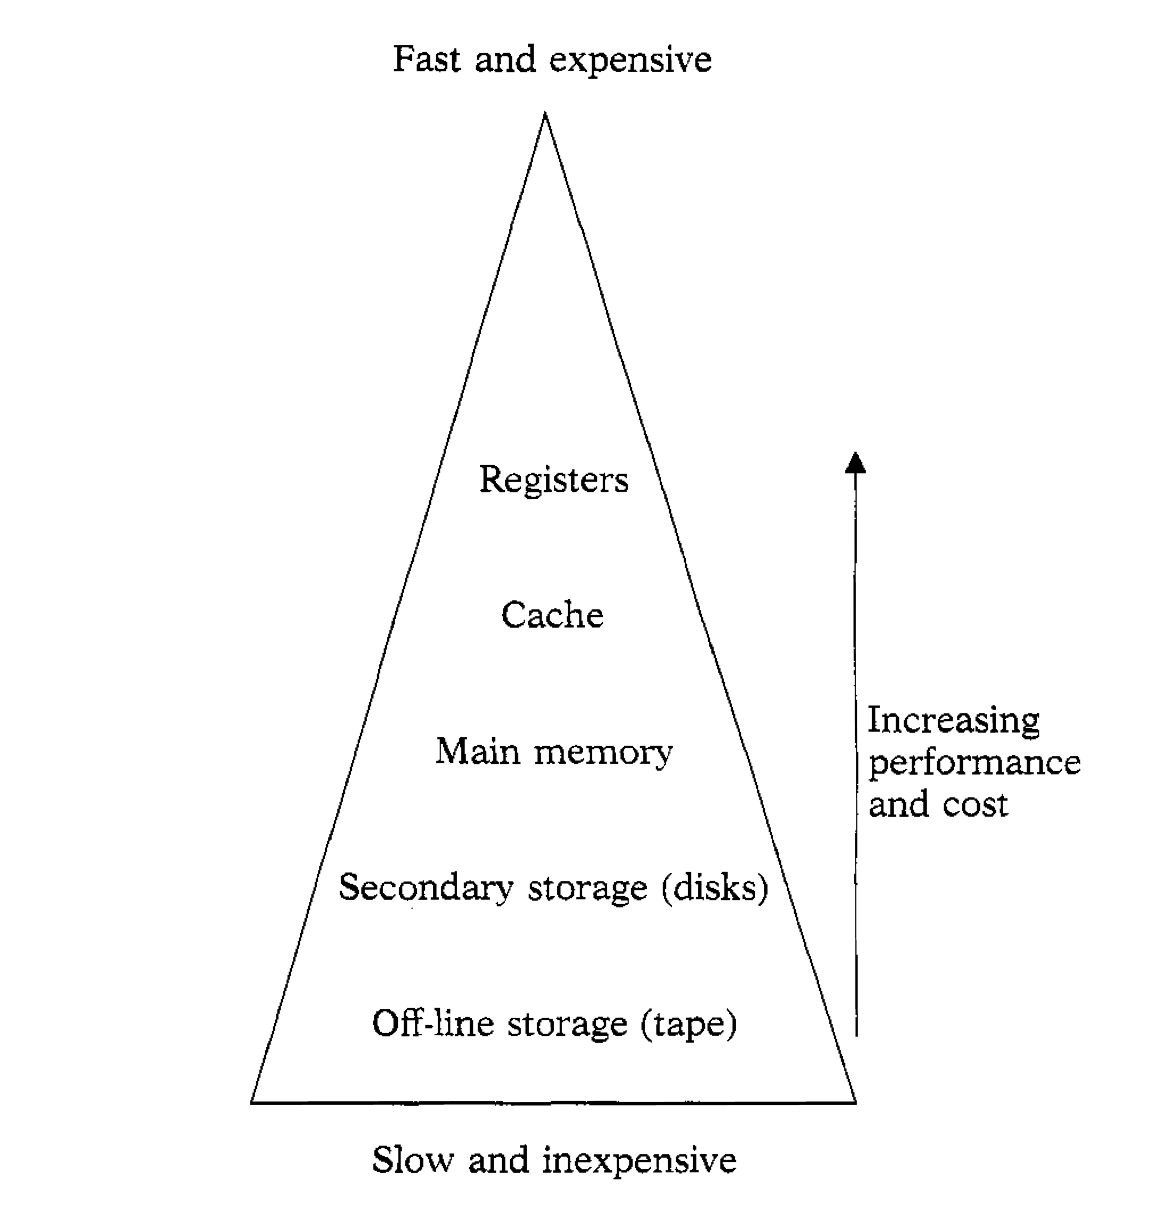
\includegraphics[width=6cm]{memHier.png}
    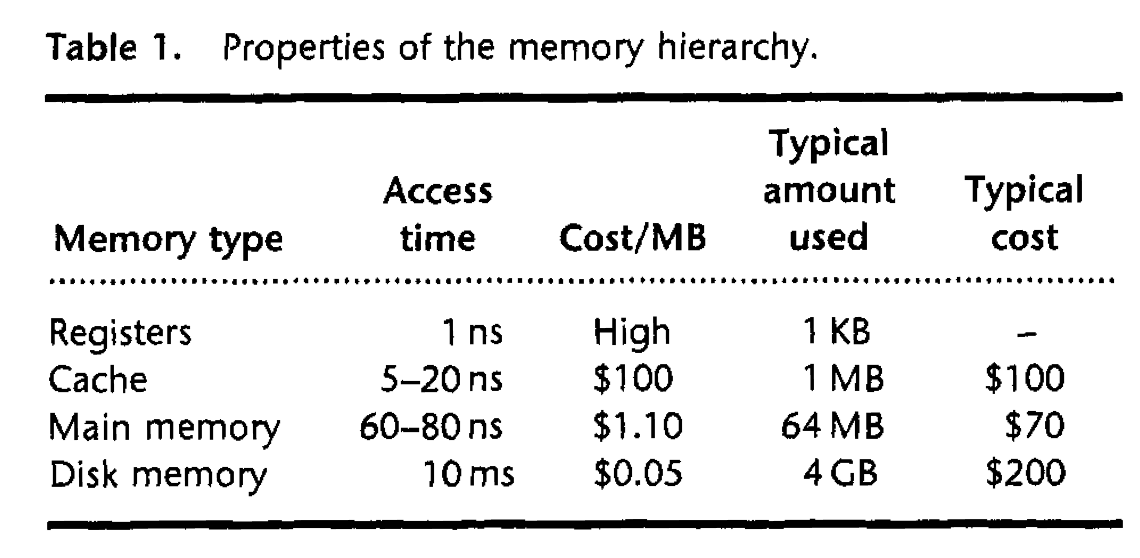
\includegraphics[width=9cm]{memTable.png}

    \cite[Murdocca et al.]{Murdocca}
\end{center}

As demonstrated in the figures above from Miles J. Murdocca et al. \cite{Murdocca}, we see that we get radically better performance the closer we access memory to the CPU.
If we design our algorithm to be more cache-efficient, then we expect massive speed-ups in practie. 

Note, when discussing page faults in this section, we will only discuss the page faults caused due to accessing the underlying bit vector of the bloom filter.
Natuarlly, page faults can occur while running the underlying code of the bloom filter, but this should be rare and would realistically cause at most one page fault.
We will now compute the expected number of page acceses for both the standard and hierarchical implementation.

The problem with doing an anaylsis on page faults is that it impossible to know when accessing a page will cause a page fault as this is dependant on the operating system and hardware.
Generally, the more memory you are using, the higher the likelyhood a page fault will occur.
In this analysis we will assume more page accesses is coorelated with a higher liklihood of page faulting.
In otherwords, we can approximate the liklihood of page page fault to the expected number of different pages that will be accessed during an operation.

First, we will discuss the standard implementation. Let $A$ be a random variable representing the number of pages accessed. 
Let $P$ be the number of bits in a page and let $m$ be the number of bits in the underlying bitvector.
Suppose there are $k$ hash functions.
We now define the indictor variable $A_i$ which is $1$ if bit $i$ is set, $0$ otherwise.
$$A = A_1 + A_2 + \ldots + A_{m/P}$$
Thus, the expected number of distinct pages accessed can be found by computing the expected value that any given page is accessed and applying linearity of expectation:
$$E(A) = \sum_{i=1}^{m/P} E(A_i) = \frac{m}{P} \cdot E(A_i) \text{ for arbitrary $i$}$$
The probability that $A_i$ is accesed at least once is the inverse of it being never accessed.
Assuming that our hash function is uniform, we expect it to pick any particular page with probability $\frac{1}{m/P} = \frac{P}{m}$.
Thus, the probablity $A_i$ is accessed at least once is:
$$E(A_i)  = 1 - (1 - \frac{P}{m})^k$$
Ergo, we have a closed form equation for the expected number of page faults for a given operation:
$$\text{Expected distinct pages accessed (Standard)} = \frac{m}{P} (1 - (1 - \frac{P}{m})^k)$$

We will use this formula to compute the expected number of page faults for two reasonable cases.
First, suppose you wanted a bloom filter to store $32,768$ elements with an underlying bit vector of size $\times 10$ that.
Note, most computer systems have a page size of $4096$ bytes, so this works out to require exactly $10$ pages of memory.
Additionally, suppose we pick the optimal bloom filter parameter and set $k=7$.
Under this scenario, we anticpate:
$$\text{Expected distinct pages accessed (Standard)} = 10(1-0.9^7) \approx 5.2$$
If we wanted to store $327,680$ elements under a similar setting, then the number of pages faults would be:
$$\text{Expected distinct pages accessed (Standard)} = 100(1-0.99^7) \approx 6.8$$

As we can see, even using a relatively small bloom filter, we anticpate almost every bit to be located in an entirely different page.
This means we can page fault multiple times during a single operation.

We will now anaylze the hierarchical implementatin. Our implementation limits bit setting and reading to a single page per insertion or query. Therefore, we access exactly one page!
$$\text{Distinct page accessed (Hierarchical)} = 1$$

Thus, our proposed hierarchical solution page faults at most one time!
Therefore, we anticpate much better performance.
\subsection{False Positive Rate}

In this section we will demonstrate that both implementations will have the same false positive rate in theory.
\subsubsection{Standard False Positive Rate}

As we have covered in class, the false positive rate of a standard bloom filter is as follows.
\begin{equation}
    (1 - (1 - \frac{1}{m})^{nk})^k \approx (1  - e)^{kn/m}
\end{equation}

Setting $k=7$ will minimize the false positive rate, as discussed in class.

\subsubsection{Hierarchical False Positive Rate}
Suppose we have a allocated $m$ bits in total chunked into bit vectors of size $P$ and that we have to inserted $n$ elements into our bloom filter.

We now want to compute the false positive rate of the hierarchical implementation.
This can be computed by supposing the bloom filter has been filled with $n$ elements and computing the probability that a querying a false key would result in a true response.

Assuming our hash function is uniform, any particular sub-bloom filter is anticpated to have $\frac{nl}{m/P} = \frac{nlP}{m} $ elements in it.
There are $m/P$ bloom filters and we choose $l$ of them to check. As before $k$ is the number of hash functions a particular bloom filter uses.
Thus, the chance any one bloom filter is set is:
$$(1-(1 - \frac{1}{P})^{lknP/m})^k$$
For our hierarchical implementation to return true, all $l$ bloom filters selected must return a positive result.
Thus, the false positive rate is:
$$((1 - \frac{1}{P})^{lknP/m})^{kl}$$
We can use a well known identity for $e^{-1}$ to approximate this false positive rate:
$$\approx (1 - e^{-lkn/m})^{lk}$$

Interestingly, this removes the dependence on the page size.
However, it is important to note that the Euler identity is $e^{-1} = \lim_{x\rightarrow\infty}(1-\frac{1}{P})^P$, so this identity fails as an approximation the smaller $P$ becomes.
Therefore, we should pick $P$ to be the largest value where we expect speed ups, which would be the size of a physical page.
More importantly, this formula becomes isomorphic to the false positive rate for the standard implementation.
If we let $k' := lk$ we see that our false positive rate for the hierarchical implementation is:
$$\approx (1 - e^{-k'/m})^{k'}$$
Therefore, as discussed for the standard implementation, the optimal selection for $k'$ is $7$.
Therefore, either $l=1$ and $k=7$ or $l=7$ and $k=1$.
Since our goal is reduce the number of pages accessed, the former is a more sensible choice.

Therefore, the best parameter selection for our hierarchical implementation would be to select $1$ bloom filter the size of a bloom filter and set $7$ bits in each one.
$$l = 1\text{ ; } k = 7$$

\subsection{Conclusion}
Our theoretical work has justified the claim that we expect this implementation to be more performant while having the same positive rate as the standard implementaiton.
Moreover, we have found the optimal parameters to use for our implementation.